\chapter{Analysis of an interesting AME region: $\lambda$~Orionis}
\label{ch:lori}

 \section{An interesting AME region}
		The $\lambda$~Orionis molecular ring, also known as the Meissa Ring is a massive stucture surrounding the $\lambda$~Orionis O-type star. The ring contains an HII region, ionized by LOri itself and its OB associates \citep{murdin77}. What had been thought of as a star\-forming region of missing molecular gas. At the time \cite{murdin77} even speculated that this could be evidence of an alternate star\-formation pathway, writing: ``Notably we need to know if $\lambda$Ori is an example of a different mode of star formation or [...] simply a case in which the progenitor molecular cloud was exhausted within the last one or two million years.''

    \cite{maddalena86,maddalena87}.  (and references therein) noted a ring of material likely being pushed out by the central, historically well-known $\lambda$~Orionis Association of B-type stars and surrounding HII reigon.

   \subsection{Where does the ring come from?}
    \cite{cunha96} argued that the ring may have resulted from a supernova explosion, further speculating that LOri may have been a companion of the progenitor. $\lambda$~Orionis is a known binary system, however its current companion is the a B-type star. \citep{murdin77}
  .
     The central region is heated by the $\lambda$~Orionis star itself, and the Orion~OB association it belongs to \citep{ochsendorf15}. The region is known to host several young stellar and protostellar objects \citep{koenig15}.

    At approx. 10$^{\circ}$ wide, we can see the outline of the structure even in the low (1$^{\circ}$ FWHM) resolution PCAME map. The ring shape itself is thought to originate from a supernova, or perhaps combined effects of the entire star formation history of the $\lambda$~Orionis Association, including the formation of its surrounding HII region \citep{aran09}.

  \subsection{A well-studied region}
    Although the $\lambda$~Orionis region has been a popular target for study since approximately the 1980s.\cite{duerr82} wrote of the relative lack of work on the overall region: ``Surprisingly, this interesting complex has been little studied''. While this seems surprising given the numbe of works on the region in the literature now, it is really the advent of all-sky missions that have driven more recent interest.  The large angular size is such that all-sky surveys were a natural boon for study of such extended structures. WISE especially was a huge source of insight \citep{koenig15}. More recently, \cite{planck15XXV} strongly highlighted the region as a strong candidate for further AME investigation.

\section{Investigative approach}
  We have carried out an initial comparison of the AME of this region with its mid to far-IR dust emission. The region is shown in Fig.~\ref{fig:orionis-akari9} as it appears in 1$^{\circ}$-smoothed A9 data.
      \begin{figure}
        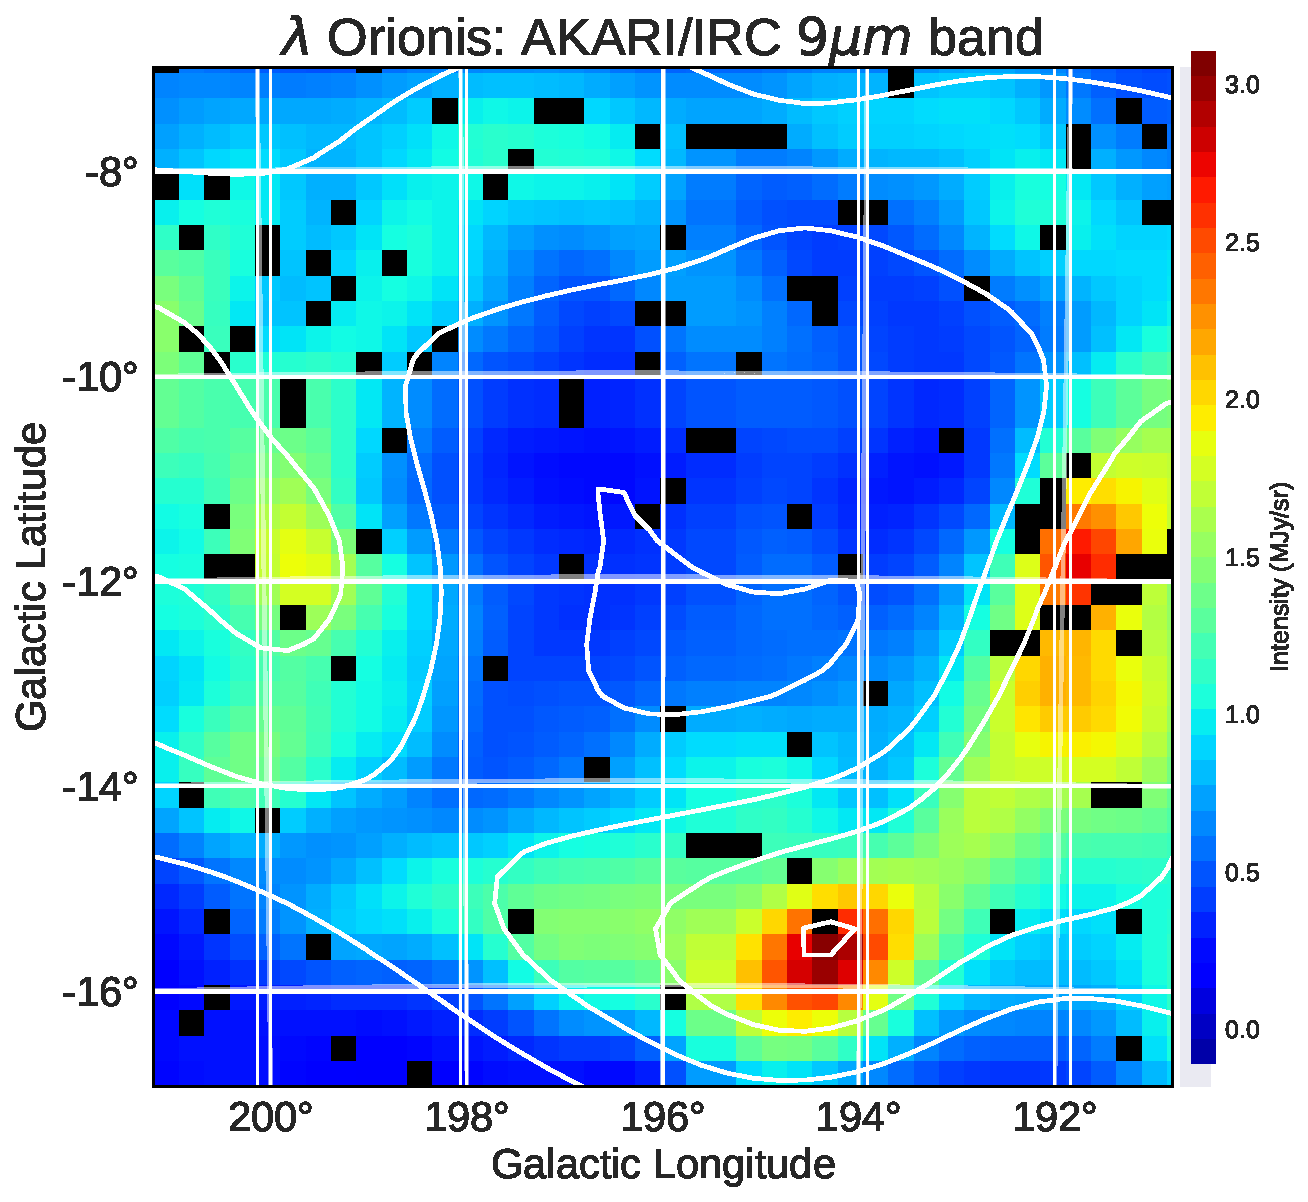
\includegraphics[width=\textwidth]{../Plots/LOri_akari9_AMEcont_1dres.pdf}
        \centering
        \caption{$\lambda$~Orionis as it appears in the AKARI 9~$\mu$m data. Contours indicate the AME, as given by the Planck PR2 AME map. The image is smoothed to a 1$^{\circ}$ PSF (much larger than the original 10 arcsec map). The $\lambda$~Orionis star itself is approximately located at the center of the image.}
        \label{fig:orionis-akari9}
      \end{figure}
      Images at each wavelength used here are included as in appendix to this thesis.
   The ring structure itself indicates excess microwave emission attributed to AME (white contours) while the central region is dominated by free-free emission \citep{aran09, koenig15}. Free-free emisison coming from the Hii phase surrounding the $\lambda$~Orionis association dominates the region's morphology in LFI images. \citep{planck15XXV}. Taking the hint from \cite{planck15XXV} that this may be among the more reliably component separated regions, we evaluate if there is any preferential relationship between any parameter of dust emission and the AME.

	\section{Data preparation}
		As indicated in Ch.~\ref{ch:datasources}, we use 12 photometric all-sky maps. For the IRC data (A9 and A18), we produce mosiacs of $\lambda$~Orionis from the individual tiles provided in the internal all-sky archive.
      \footnote{IRC all-sky data is still in the proprietary phase at the time of this writing, but should be public by April 2018.}
       For the other sources, HEALPix all-sky maps are available publicly, at sufficient resolution relative to their native resolutions. \footnote{Planck data was retreived from the NASA IPAC online archive at \url{http://irsa.ipac.caltech.edu/data/Planck/release_2/all-sky-maps/}}\footnote{AKARI/FIS data }\footnote{IRAS/IRIS data }

		\subsection{Extraction from HEALPix maps}
		  For the data obtained via HEALPix maps, we employ the ``healpix2wcs'' functionality provided in the ``gnomdrizz'' python package\footnote{Available at \url{http://cade.irap.omp.eu/dokuwiki/doku.php?id=software}}\footnote{``drizzlib'' 1.2.2 and earlier were not able to correctly access HEALPix files with multiple fields/columns. See appendix for our recommended workaround.} A9 and A18 images are produced by regridding the images with the ``montage'' software by NASA/IPAC. All of the images for all of the bands are based on a common FITS header which has a pixel grid spacing equal to the average pixel width in the NSIDE 256 HEALPix scheme.
      A background estimation and subtraction is made

      \subsection{Point-source and artifact masking}

      \subsection{PSF Smoothing}
        \begin{lstlisting}[language=Python]
          import numpy as np

          def incmatrix(genl1,genl2):
              m = len(genl1)
              n = len(genl2)
              M = None #to become the incidence matrix
              VT = np.zeros((n*m,1), int)  #dummy variable
        \end{lstlisting}

      \subsection{Background subtraction}
         We estiamte an average, flat background level for this region. Although this region is far from the Galactic plane, there is an appreciable background level which must be subtracted. We define two standard background `OFF` zones, indicated in Fig.~\ref{fig:lori_bgsep}, and use these to determine mean, flat background level. We do not expect the band-by-band correlation tests with the AME to be sensitive to this background subtraction

		\section{Multi-wavelength characterization}
			Figure~\ref{fig:orionis-img} shows the region in 12 photometric bands, from the mid to far IR, covering key dust emission regimes as described in Ch.~\ref{ch:datasources}.
        \begin{figure}
          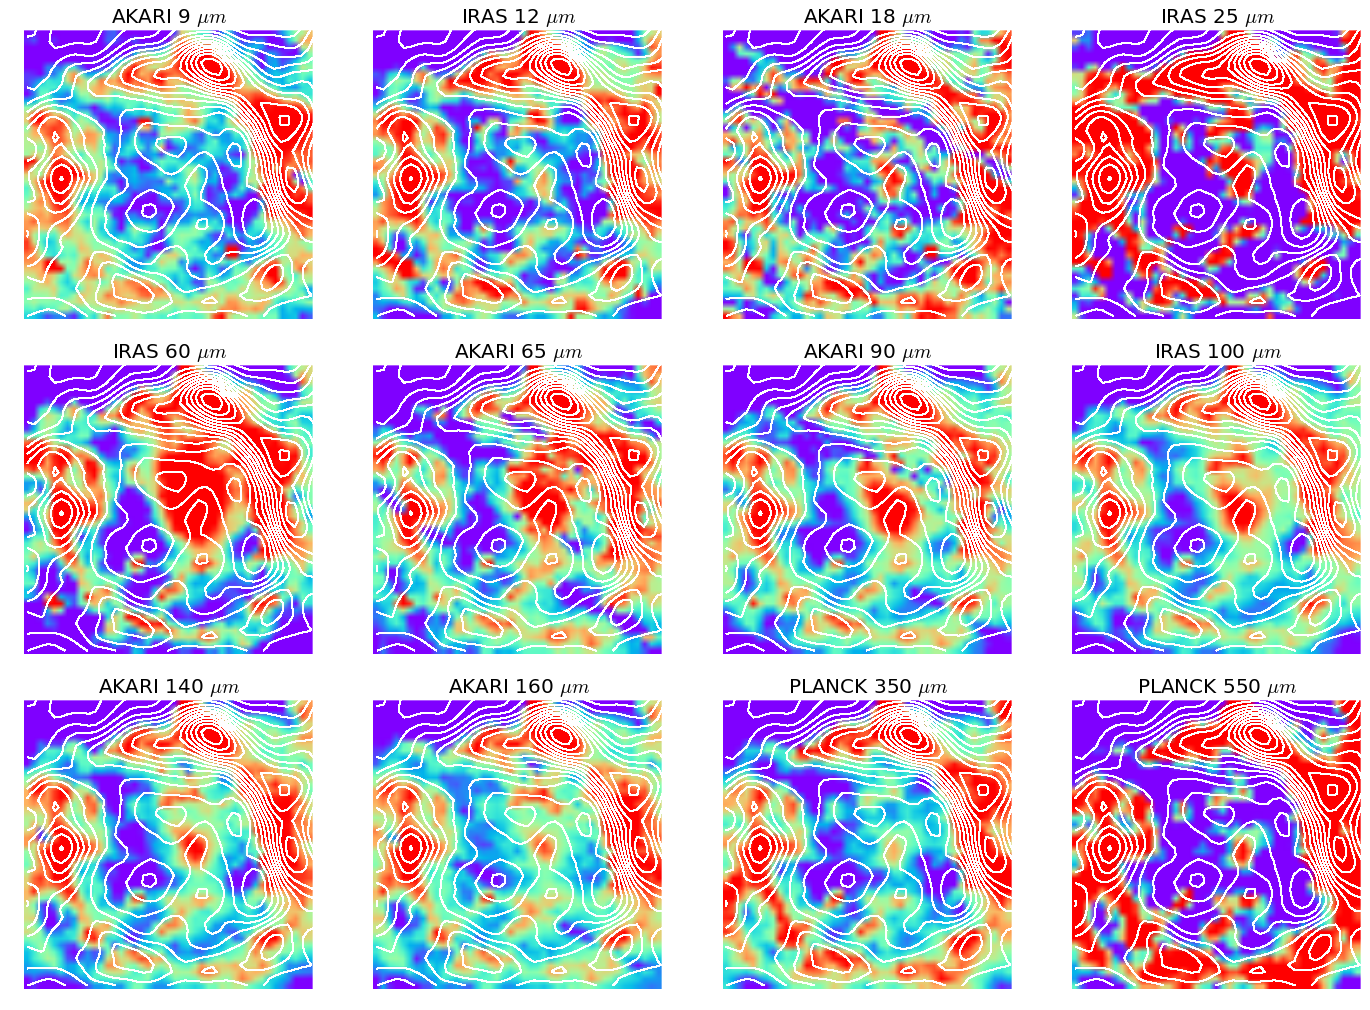
\includegraphics[width=\textwidth]{../Plots/lOrionis_grid_img.png}
          \centering
          \caption{A grid of thumbnails showing the $\lambda$~Orionis region's structure, at 12 wavelengths, along with AME contours (shown in white countours. Spatial correlation seems to be the best at the shortest and longest wavelengths (AKARI/IRC 9~$\mu$m and Planck/HFI 550~$\mu$m). The images are smoothed and interpolated for demonstration. Figure~\ref{fig:orionis-akari9} demonstrates the actual pixel grid used for the SED fitting and intensity correlation tests.}
          \label{fig:orionis-img}
        \end{figure}
			Contours indicate the region's shape in the PCAME map. Figure~\ref{fig:orionis-corr} shows IR to AME cross correlation plots, for all pixels within the 10$^{\circ}$ by 10$^{\circ}$ $\lambda$~Orionis region.
        \begin{figure}
          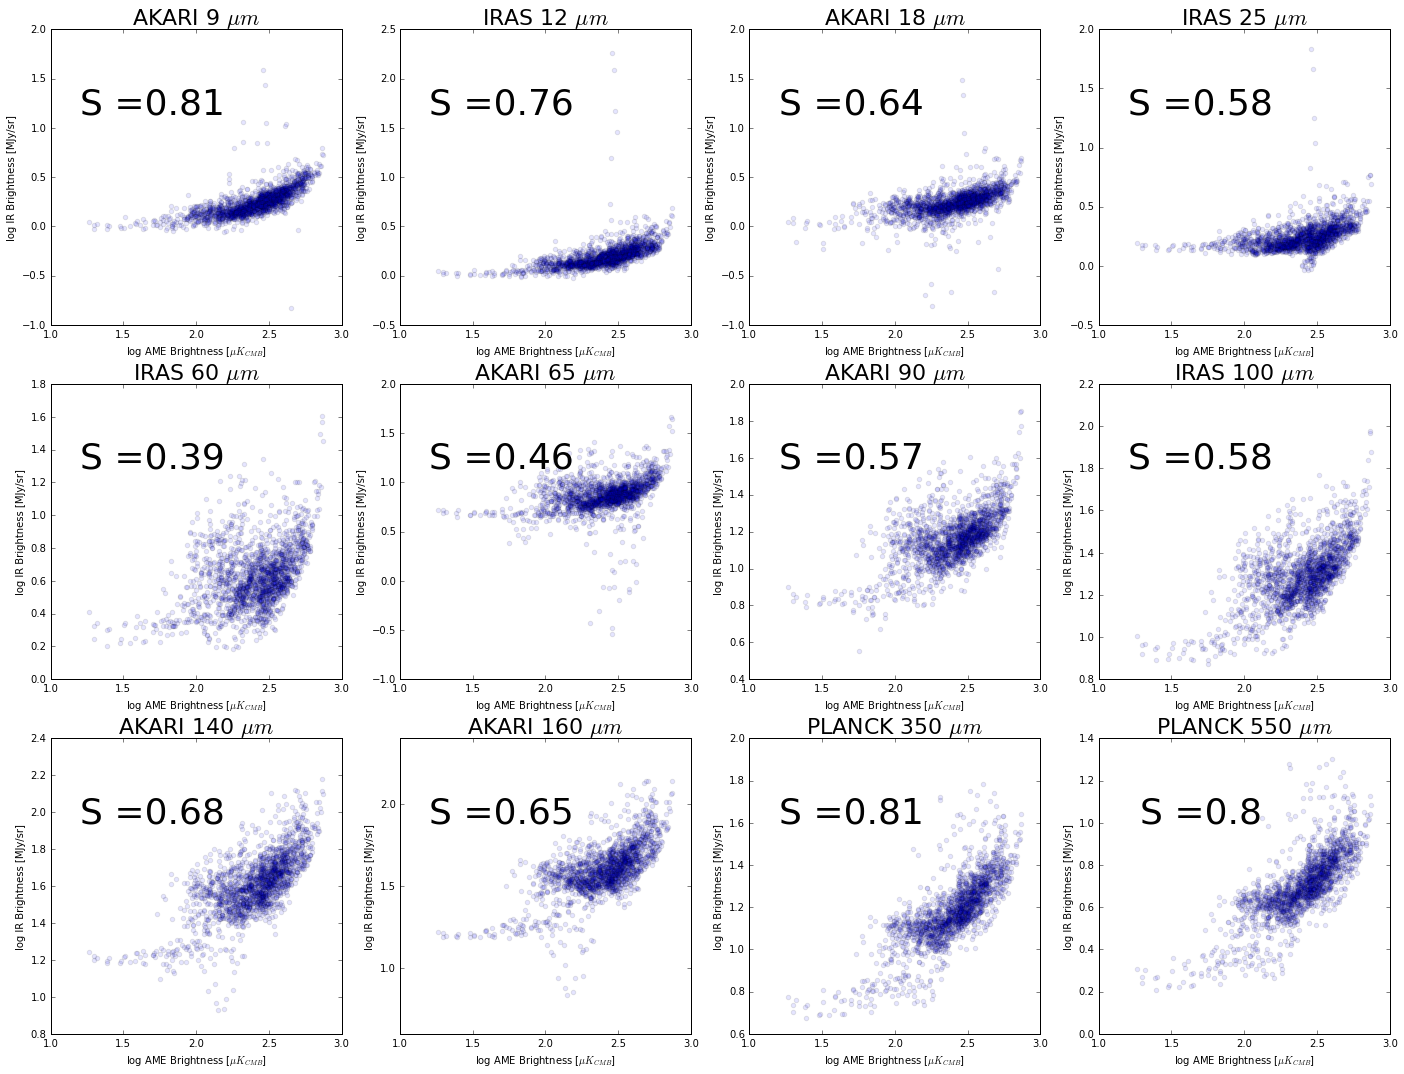
\includegraphics[width=\textwidth]{../Plots/orionis_correlations_AME.png}
          \centering
          \caption{Intensity cross-correlation for all pixels in the $\lambda$~Orionis cut-out region.  $r_{s}$ indicates the Spearman rank correlation coefficient for each plot.}
          \label{fig:orionis-corr}
        \end{figure}
    The correlation matrix results corresponding to data shown in Fig.~\ref{fig:orionis-corr}, are shown in Fig.~\ref{fig:orionis-corr-matrix}.
        \begin{figure}
          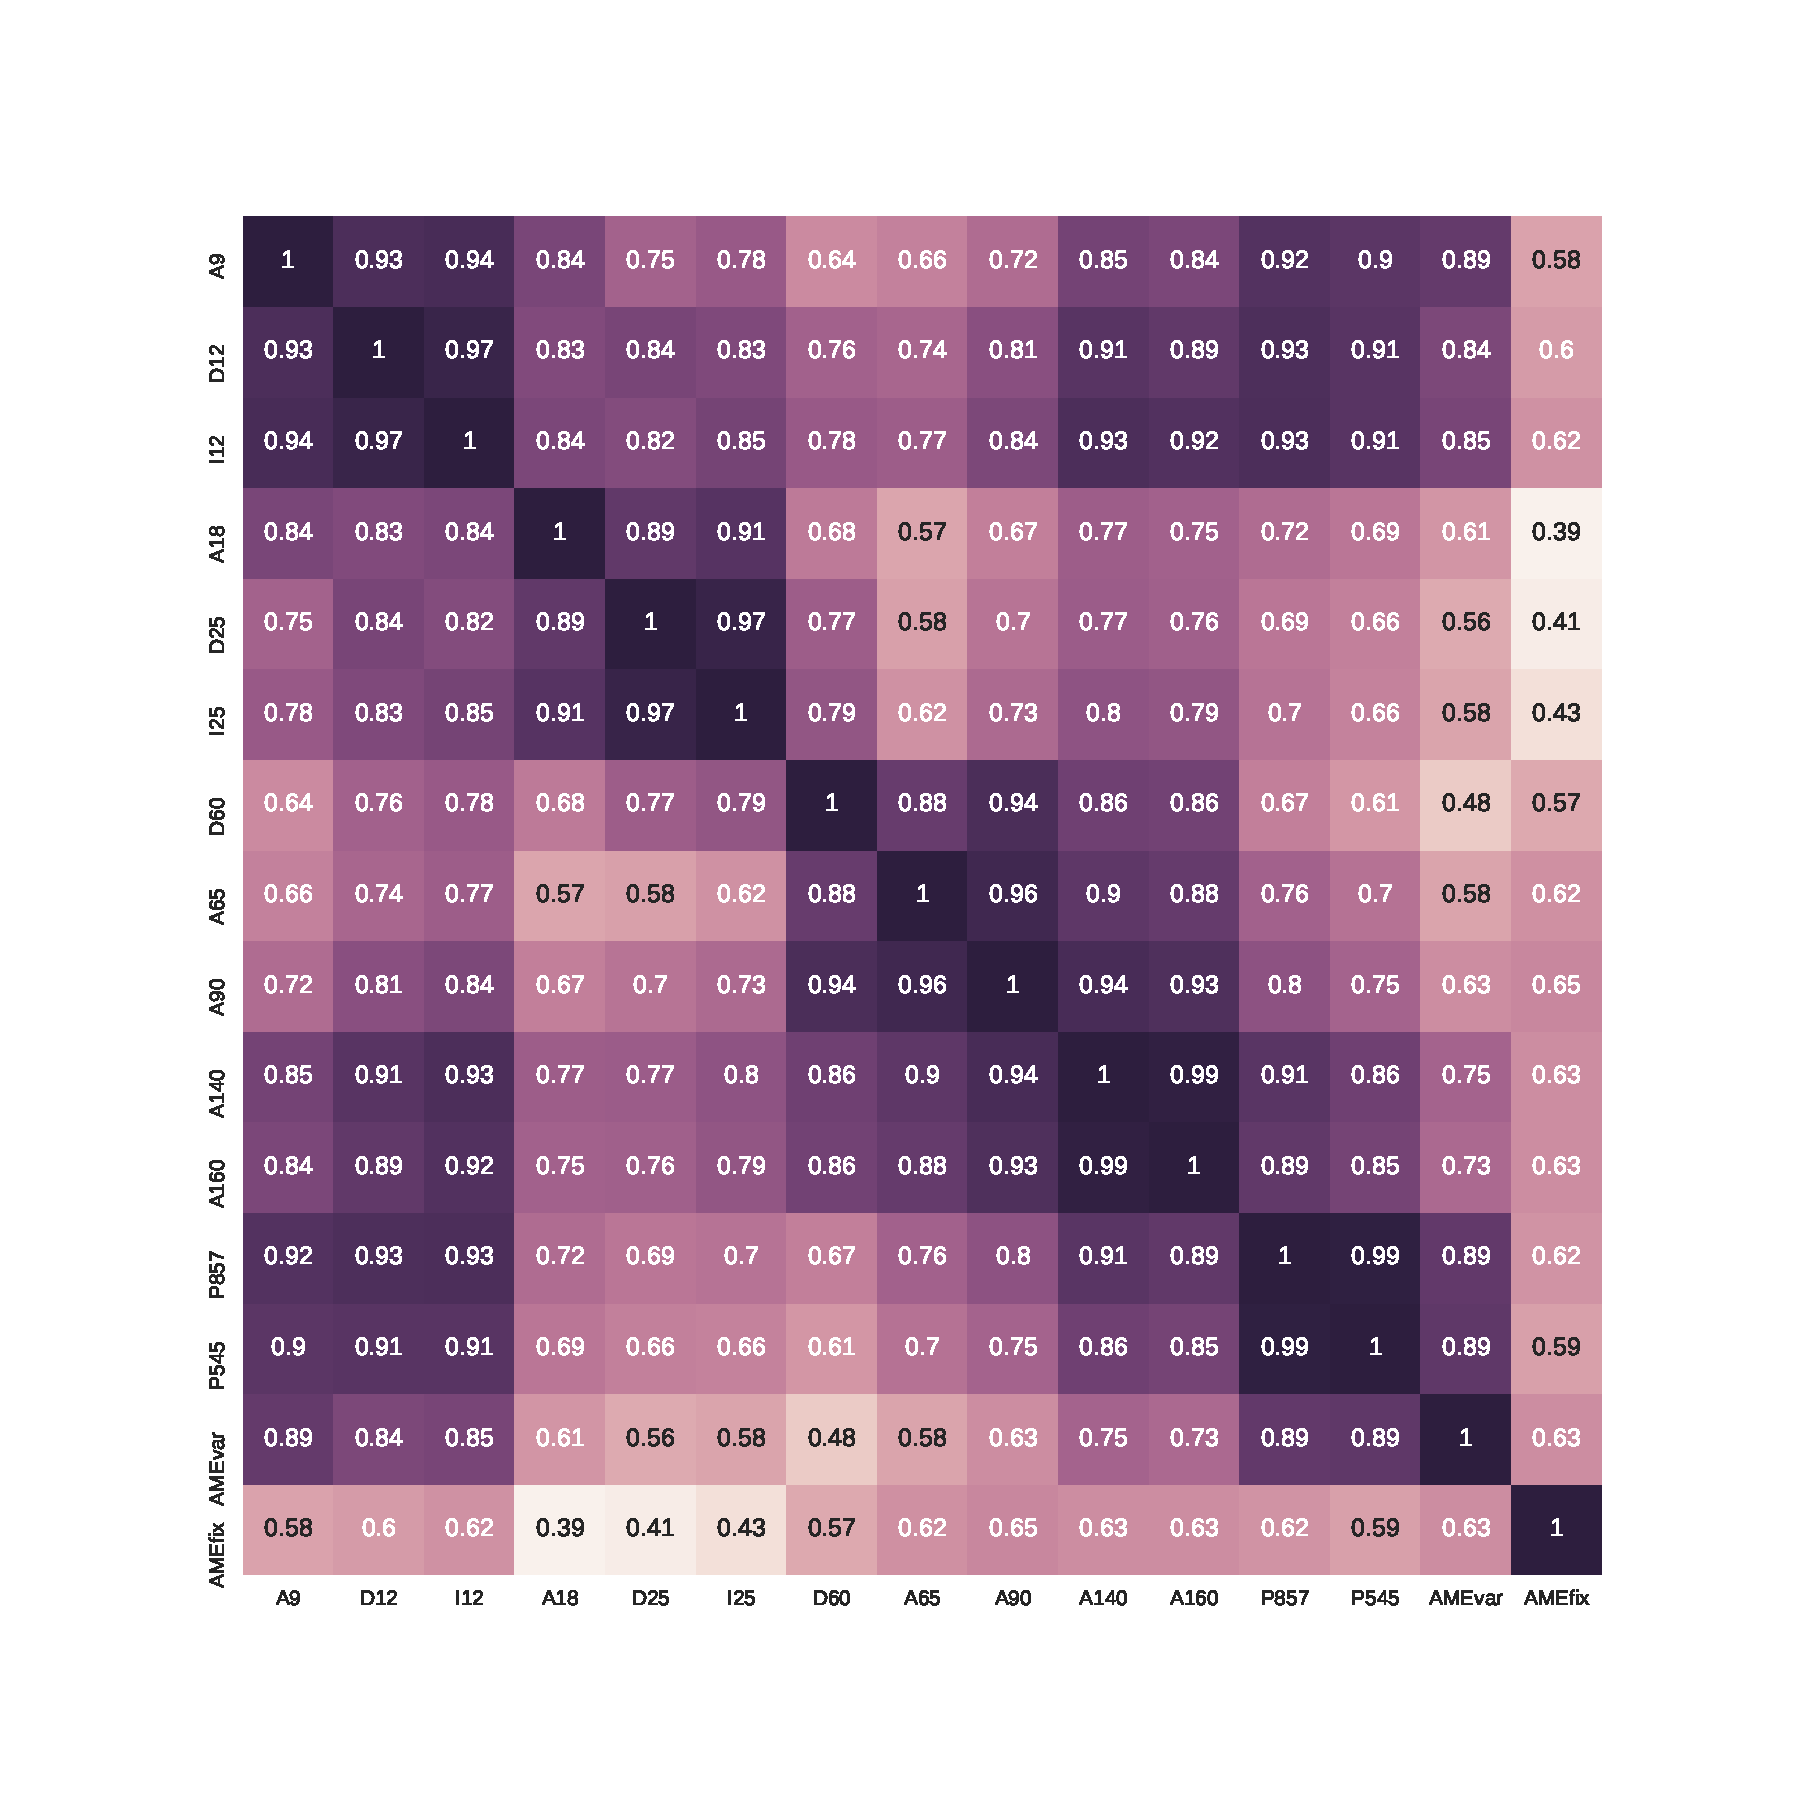
\includegraphics[width=\textwidth]{../Plots/ch_lori/Lori_corrmatrix_I.pdf}
          \centering
          \caption{$r_{s}$ correlation matrix for all of the data used in the $\lambda$~Orionis analysis.}
          \label{fig:orionis-corr-matrix}
        \end{figure}
    The correlation is most clear for the shortest and for the longest wavelength bands, and weakens the most at around 60~$\mu$m. The weakening of the correlation score appears to come from brighter 25 to 90~$\mu$m emission within the ring. The spectrum is consistent with warm thermal dust emission, heated by $\lambda$~Orionis and its associates. The ring structure itself appears relatively consistent accross all of the IR bands.
    \subsection{Bootstrap analysis}
        To assess the robustness of the correlation scores, we employ the Bootstrap re-sampling approach, first introduced by \cite{efron79}. This involves creating random re-sampled sets of the data. We use the 'with replacement' approach, meaning that a data point may be selected multiple times in a single re-sampling iteration. The size of the re-sampled set is the same is the input set size. For each random set we run a correlation test, resulting in a distribution of correlation coefficient. This allows us to estimate error bars for the correlation scores.
        We carry out bootstrap correlation tests for each IR band's intensity vs. the AME intensity. The data are resampled 10,000 times for each correlation test. This is repeated for both $r_{s}$ and $r_{p}$ based tests. The distributions of the boostrap resamplings are show in in Fig.~\ref{fig:bootstrap_vs_AME}.
            \begin{figure}
              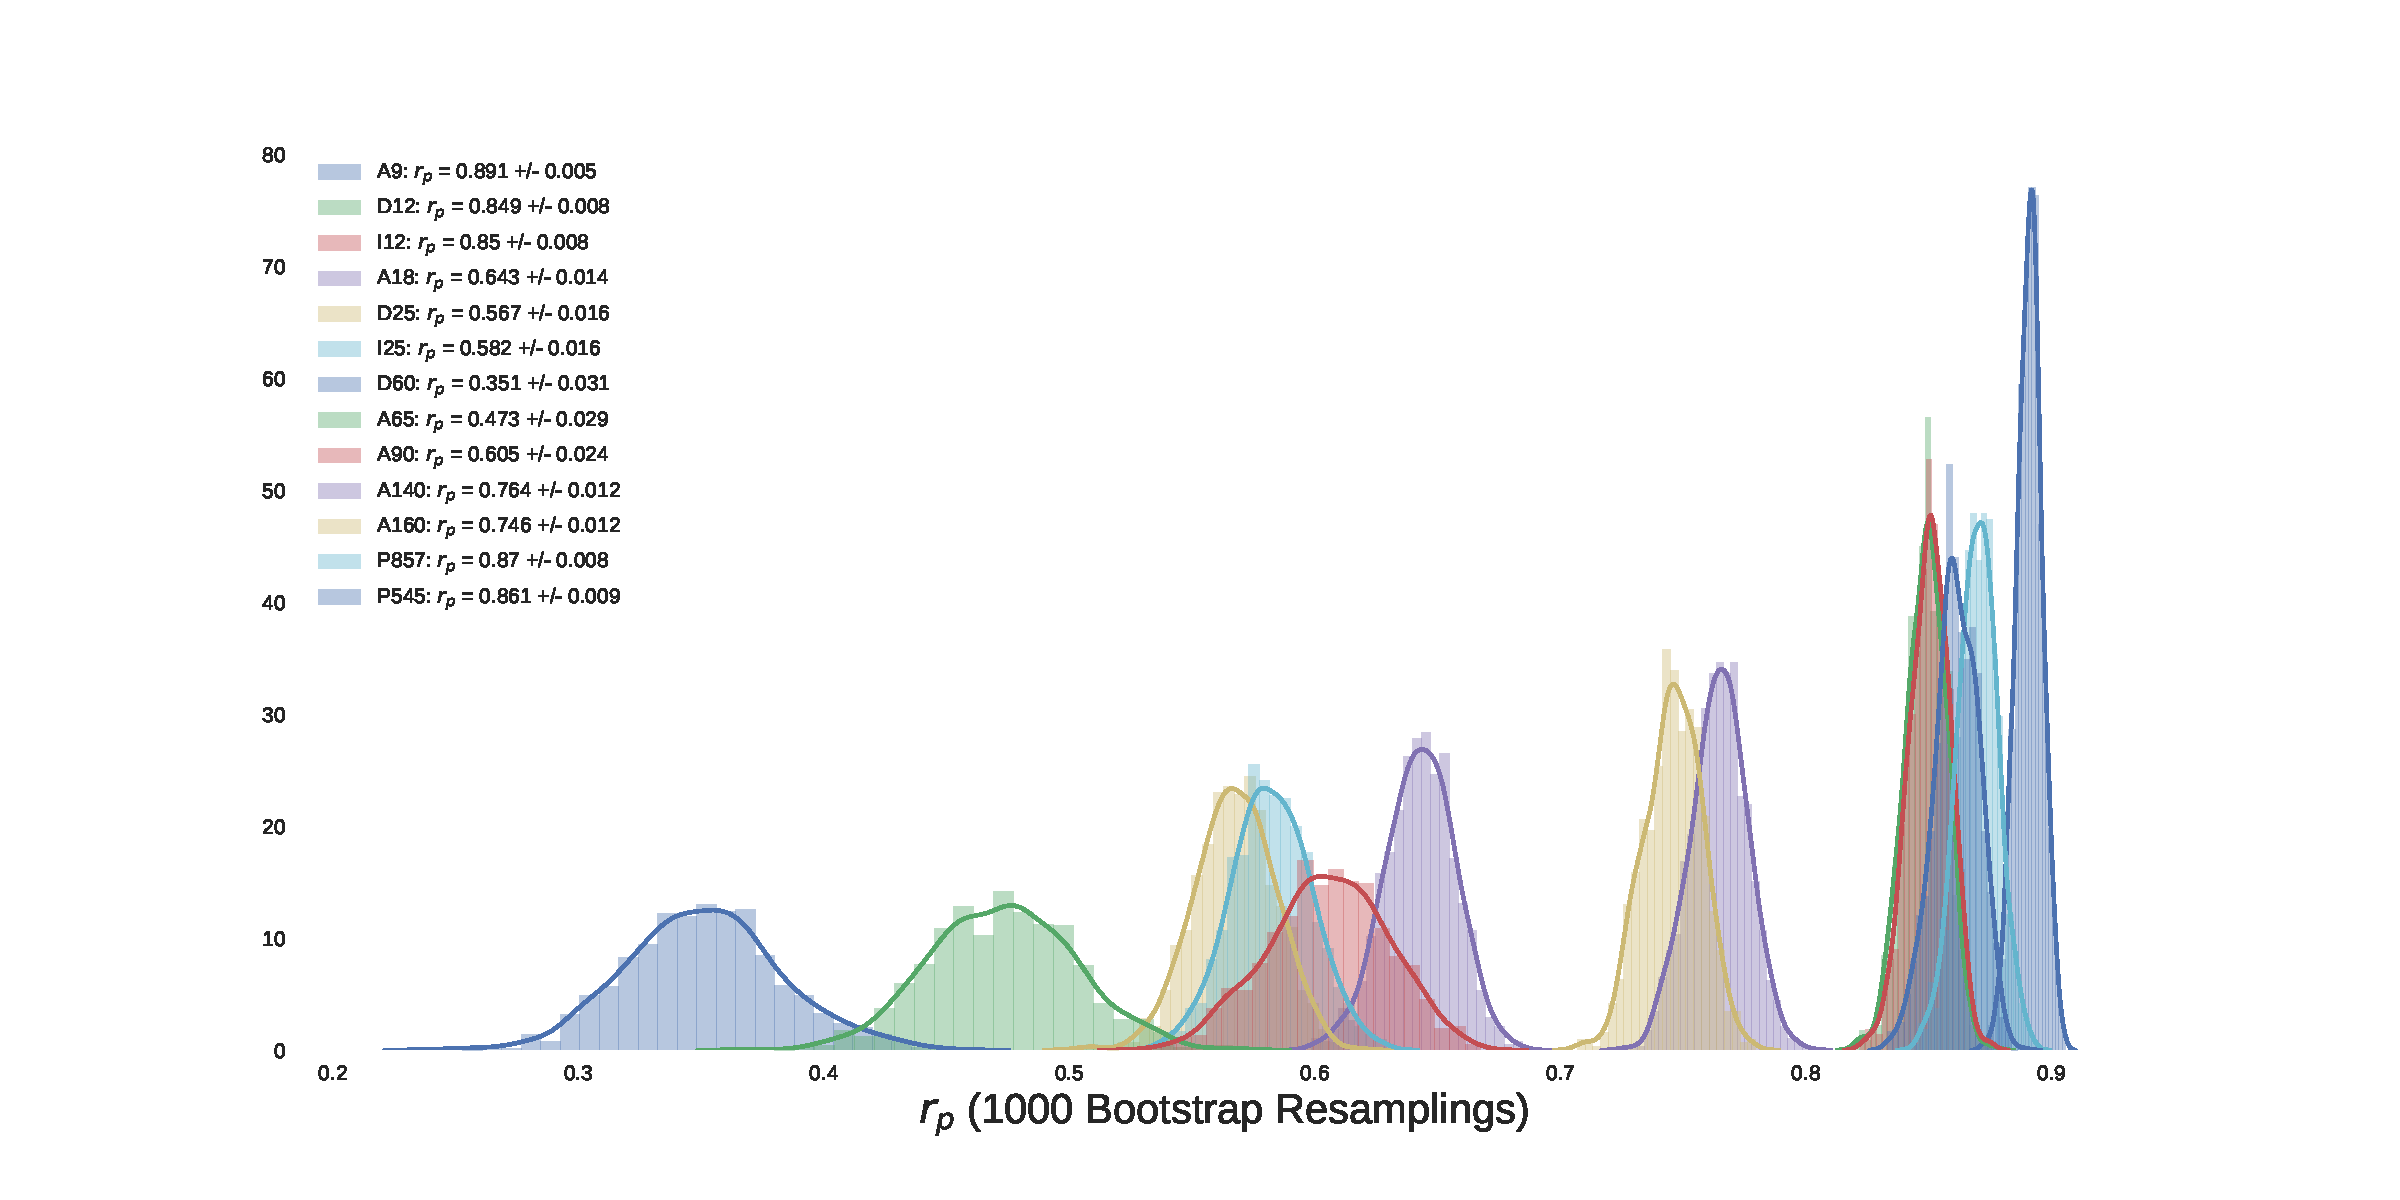
\includegraphics[width=\textwidth]{../Plots/ch_lori/bootstrap_vs_AME_pearson_i1000.pdf}
              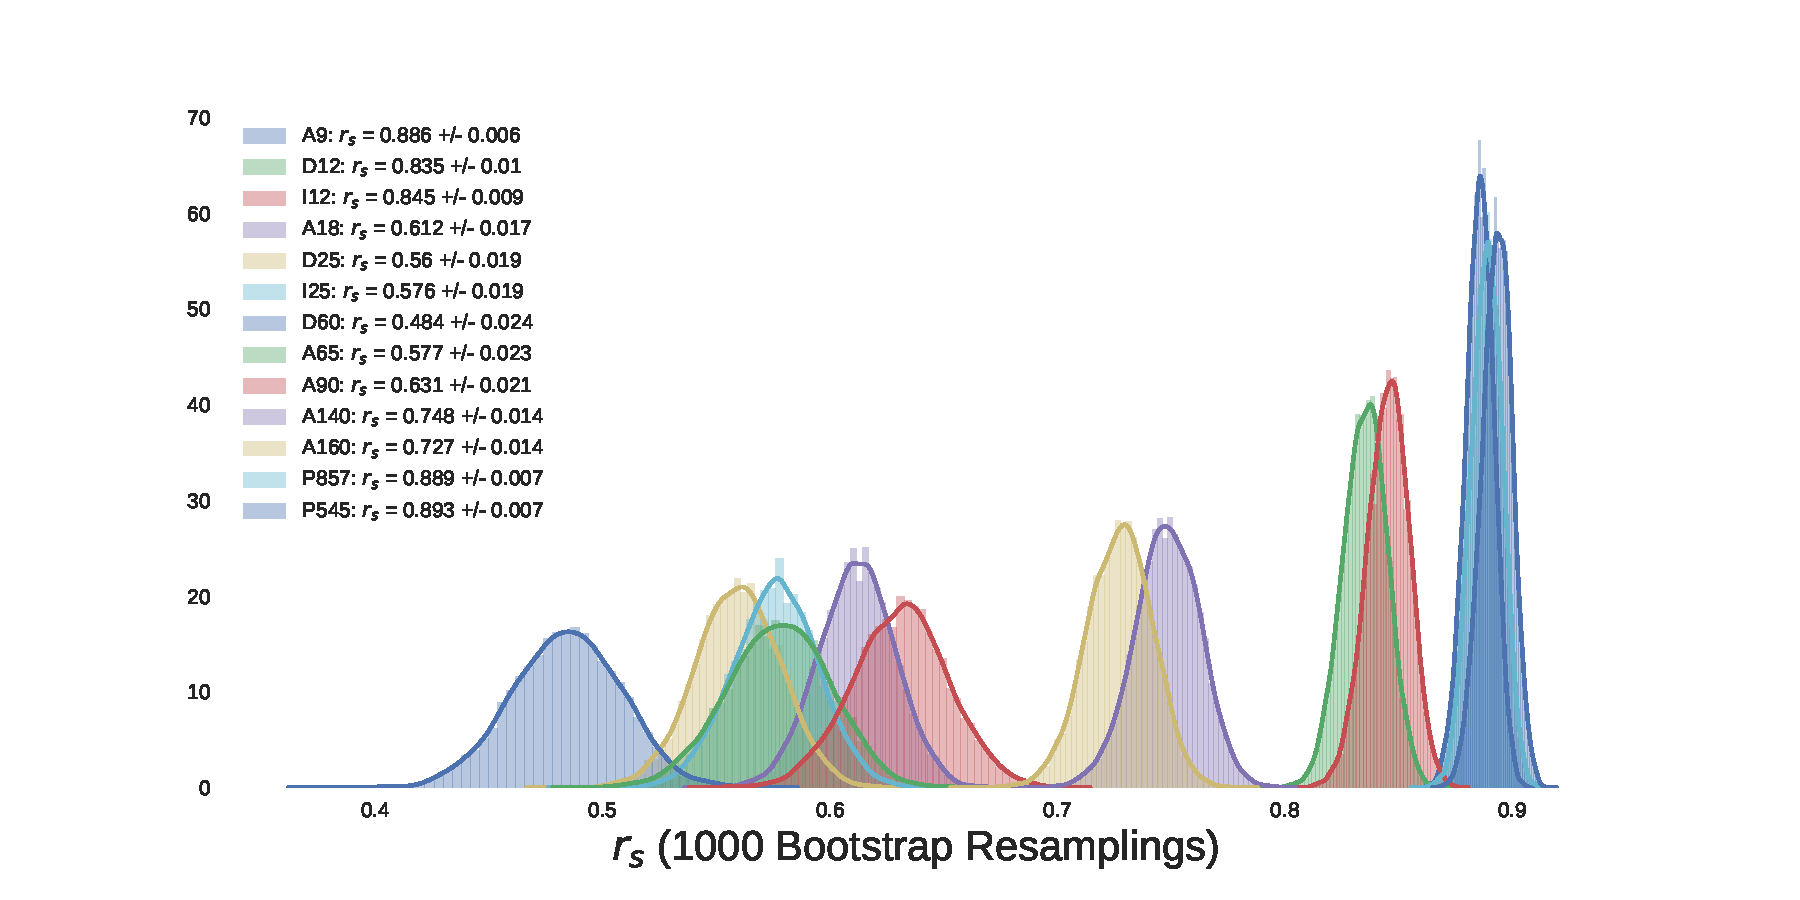
\includegraphics[width=\textwidth]{../Plots/ch_lori/bootstrap_vs_AME_spearman_i1000.pdf}
              \centering
              \caption{Re-sampled (Bootstrap) correlation tests for IR emission in $\lambda$~Orionis vs. AME, for both Spearman and Pearson correlation tests.) }
              \label{fig:bootstrap_vs_AME}
            \end{figure}
        For both test cases, the best correlations are the longest and shortest wavelength bands. In the $r_{p}$ case, the strongest correlation is the A9 band vs the AME.
        \section{Comparison with SED Fitting}
          We performed a full dust SED fitting on the $\lambda$~Orionis photometry, according to the dust model by \cite{galliano11} (to be thoroughly introduced in Galliano, et al., in prep.)  We used a mixture of silicate and carbonaceous dust, silicate dust, the two dominant categories of interstellar dust as described in Ch.~\ref{ch:intro}. However, instead of the graphite-based carbon dust invoked by the canonical \cite{draine07} model (DL07), we assume amorphous carbon. This choice is an attempt to account for the ``sub-mm excess'' of dust emission, reported by \cite{israel10, bot10}, in the Large Megallanic Cloud (LMC). The increased emissivity of amorphous carbon (a factor of 2-3 more than DL07) allows a better fit to Herschel observations of the LMC \citep{galliano11}, and Planck observations of the Milky Way \citep{planckIntXXIX16}. We assume that the radiation field heating this dust mixture is the Galactic ISRF \citep{mathis83}, scaled by a factor $U$. We also assume, following \cite{dale01}, that the dust is exposed to a distribution of starlight intensity, distributed as:
              \begin{equation}
                 \label{eq:U}
                   dM_{dust}\propto{} U^{-\alpha}dU
              \end{equation}
          between $U_{min}$ and $U_{max}$, where $U_{min}$, $U_{max}$ and $\alpha{}$ are free parameters.
          We utilize both the Bayesian dust SED fitting approach by Galliano (in prep.), and a least-squares analysis. The SED fitting accounts for estimates of the respective calibration uncertainties, and the spectral response curves (Fig.~\ref{fig:Filter_coverage_example_full}). As outputs, metrics of the total dust mass $M_{dust}$, PAH mass $M_{PAH}$, ionized PAH mass $M_{PAH+}$, and ISRF intensity $U$ are produced. We only carry out the fitting for unmasked pixels. We are primarily interested in which of the corrleations $M_{dust}$ vs. $I_{AME}$ or $M_{PAH}$ vs. $I_{AME}$ is stronger.
          Two sample fitting results are shown in Figs.~\ref{fig:fred_LOri_notes_Oct2017_fig1a}, and~\ref{fig:fred_LOri_notes_Oct2017_fig1b}.
              \begin{figure}
                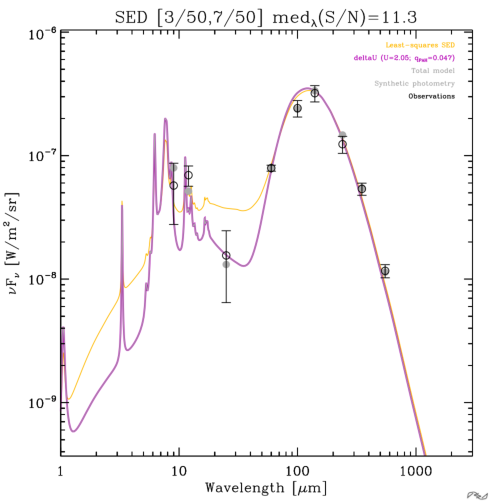
\includegraphics[width=\textwidth/2]{../Plots/ch_lori/fred_LOri_notes_Oct2017_fig1a.pdf}
                \centering
                \caption{Observed (black circles and errors) and synthetic photometry (gray dots) SED of a pixel within $\lambda$~Orionis, along with the dust SED model fit results. Two SED fits are shown: on for the Bayesian fitting (magenta), and another showing the standard least-squares result for comparison (yellow). The fitted ISRF strength $U$, and fraction of mass in PAHs, $q_{PAH}$ are also given.}
                \label{fig:fred_LOri_notes_Oct2017_fig1a}
              \end{figure}
              \begin{figure}
                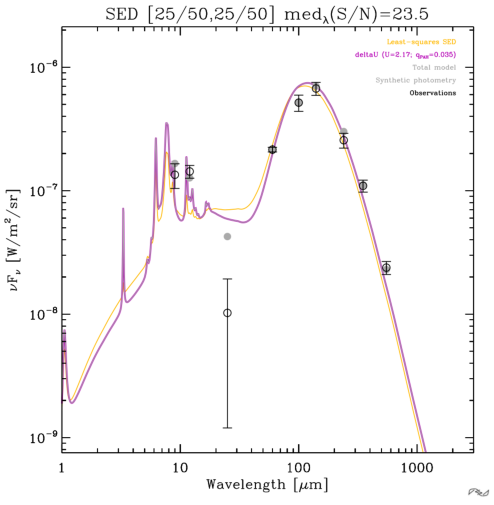
\includegraphics[width=\textwidth/2]{../Plots/ch_lori/fred_LOri_notes_Oct2017_fig1b.pdf}
                \centering
                \caption{The same as Fig.~\ref{fig:fred_LOri_notes_Oct2017_fig1a}, but for a different pixel position. Corresponds to galactic coordinates...}
                \label{fig:fred_LOri_notes_Oct2017_fig1b}
              \end{figure}
           Performing such fits for all of the pixels, we are able to see how $I_{AME}$ varies with the bulk dust physical characteristics of the region. Fig.~\ref{fig:fred_LOri_notes_Oct2017_fig2a} shows the fitted dust mass per pixel, relative to the AME intensity.
                \begin{figure}
                 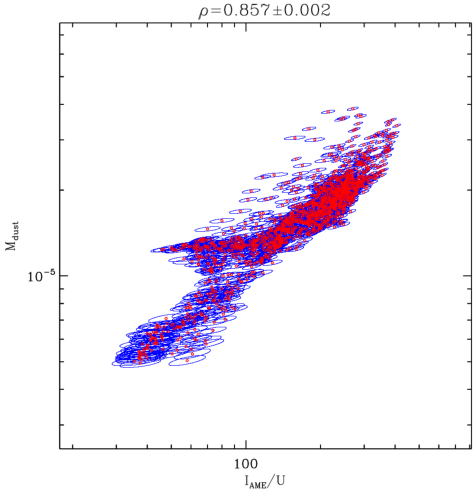
\includegraphics[width=\textwidth/2]{../Plots/ch_lori/fred_LOri_notes_Oct2017_fig2a.pdf}
                 \centering
                 \caption{Scatter plot with error elipses generated through the Bayesian SED fitting, of total dust mass $M_{dust}$ vs. $I_{AME}$ scaled by $U$.}
                 \label{fig:fred_LOri_notes_Oct2017_fig2a}
               \end{figure}
           AME intensity is scaled by the ISRF intensity $U$. Although spinning dust emission is not predicted to vary directly with $U$, we consider that the ISRF may serve as a diagnostic of environmental conditions in the ISM. In any case, we find that performing such a scaling improves the correlations with dust mass.   Figs.~\ref{fig:fred_LOri_notes_Oct2017_fig2b} and~\ref{fig:fred_LOri_notes_Oct2017_fig2d} describe the variation with $M_{PAH}$ and $M_{PAH+}$.
              \begin{figure}
                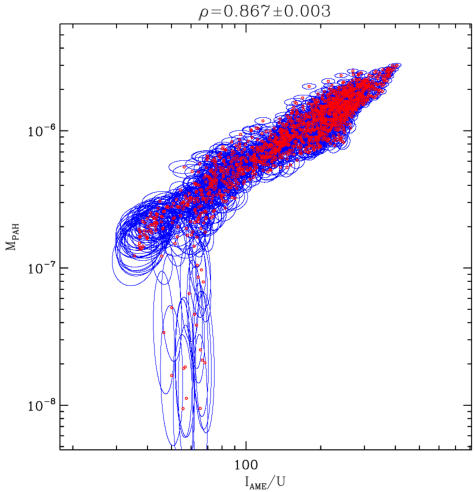
\includegraphics[width=\textwidth/2]{../Plots/ch_lori/fred_LOri_notes_Oct2017_fig2b.pdf}
                \centering
                \caption{The same comparison is given by~\ref{fig:fred_LOri_notes_Oct2017_fig2a}, but showing total mass of PAHs ($M_{PAH}$) rather than total dust mass on the y-axis. }
                \label{fig:fred_LOri_notes_Oct2017_fig2b}
              \end{figure}
              \begin{figure}
                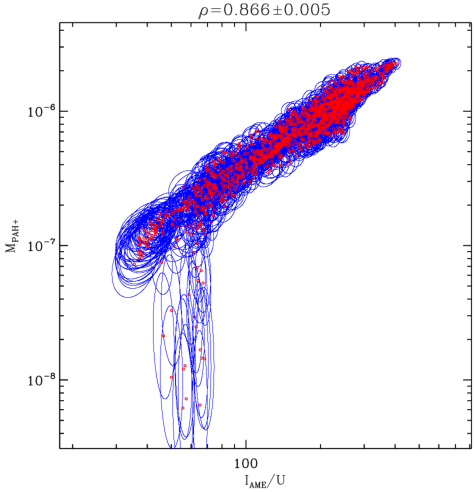
\includegraphics[width=\textwidth/2]{../Plots/ch_lori/fred_LOri_notes_Oct2017_fig2d.pdf}
                \centering
                \caption{ The same as in Figs.~\ref{fig:fred_LOri_notes_Oct2017_fig2a} and~\ref{fig:fred_LOri_notes_Oct2017_fig2b} , but specifically comparing an estimate of the ionized component of PAH mass. }
                \label{fig:fred_LOri_notes_Oct2017_fig2d}
              \end{figure}
    Based on the dust properties derived from these SED fits, we attempt investigate whether any fitted parameter shows a preferential relation with the AME.

  \section{Discussion}
    \subsection{AME:PAH}
      In  $\lambda$~Orionis we found that accross the whole region, A9 emission and P545 emission were the most strongly correlated with AME. This is apparent both in the photometric band analysis, and in the dust SED fitting.  The fact that the correlation strengths of PAH-tracing mission and sub-mm emission are similar is in-line with what we have seen in \cite{ysard10b} and \cite{hensley16}. In those works, the two relationships (MIR vs. AME and FIR vs. AME) are very close, although these two papers are odds as to which relationship is stronger, and thus in their final interpretation. With the present data and analysis of $\lambda$~Orionis, we fail to rule out PAHs as carriers of the AME. Fig.~\ref{fig:fred_LOri_notes_Oct2017_fig2c} indicates that although total dust mass and PAH mass are both correlated with AME, there is a strong (\~100\%) probability that PAH mass is the stronger predictor of AME intensity.
          \begin{figure}
            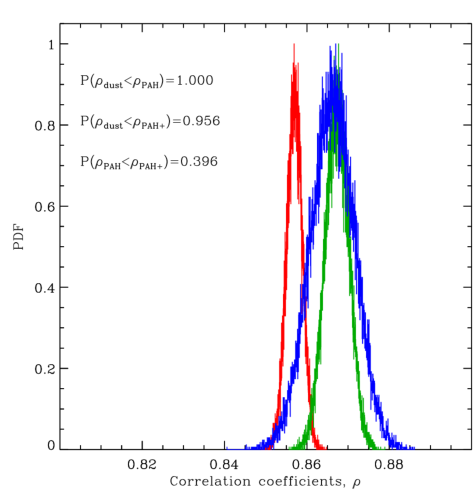
\includegraphics[width=\textwidth/2]{../Plots/ch_lori/fred_LOri_notes_Oct2017_fig2c.pdf}
            \centering
            \caption{ The Bayesian correlation probablity distributions of Pearson's correlation coeffocoemt ($\rho{}$) for the three physical parameters vs. the AME intensity: total dust mass, $rho_{dust}$ (red); total PAH mass $rho_{PAH}$ (green); and only the ionized PAH mass $rho_{PAH+}$ (blue). Also given are the probabilities of either PAH component being better correlated with AME than dust mass, as well as the probability that ionized PAH mass correlates better than total PAH.}
            \label{fig:fred_LOri_notes_Oct2017_fig2c}
          \end{figure}
        The results are consistent with a scenario in which PAH mass, cold dust, and the AME are all tightly correlated. Weaker correlation from 25 to 70~$\mu$m may indicate that AME is weaker in regions of warmer dust and stronger radiation fields. Such an anti-correlation with harsher radiation are consistent with the carriers of AME being destroyed in the central region of $\lambda$~Orionis, thus leading to substantially decreased spinning dust emission.

      \subsection{PAH Ionization fraction}
          As described in Ch.\ref{ch:datasources} it is expected that relative variationes between the A9 and I12 intensities could be explained by the fraction of PAHs that are charged. Simply examining $\lambda$~Orionis in intensity, we find that the A9 intensity correlates more strongly with AME than I12 or D12. In the Pearson correlation case, A9 correlates more strongly with AME than any other band. This is consistent with the spinning PAH hypothesis, and taken alone may that the 6.2~$\mu$m feature emission from ionized PAHs, may be a better predictor of AME intensity.

          As shown by the dust SED fitting however, the probability distributions (Fig.~\ref{fig:fred_LOri_notes_Oct2017_fig2c}) of $r_{p}(M_{PAH+}:I_{AME})$ does not indicate that ionized PAH mass correlates better with the total PAH mass. Attempts to estimate the PAH fraction based on the available data appear to only add noise relative to $r_{p}(M_{PAH}:I_{AME})$. The means of the two distrubtions $r_{p}(M_{PAH+}:I_{AME})$  and $r_{p}(M_{PAH}:I_{AME})$ are similar and $r_{p}(M_{PAH+}:I_{AME})$ shows a wider distribution.

         Thus the question of whether or not AME comes predominantly from charged PAHs remains open. The fact that A9 correlates more strongly than the 12~$\mu$m bands, at least suggests that this topic is worth further investigation. Future wide-area spectral mapping of the $\lambda$~Orionis region would be able to indicate precisely which PAH features are dominating the A9 and I12 emission, and infer the charged PAH fraction with higher confidence than we can do with wide photometric band ratios. Such observations could be coupled with higher resolution constraints of the AME variation, and a more reliable fitting of the peak frequency of the AME.
